% Options for packages loaded elsewhere
\PassOptionsToPackage{unicode}{hyperref}
\PassOptionsToPackage{hyphens}{url}
\PassOptionsToPackage{dvipsnames,svgnames,x11names}{xcolor}
%
\documentclass[
  a4paperpaper,
]{article}

\usepackage{amsmath,amssymb}
\usepackage{iftex}
\ifPDFTeX
  \usepackage[T1]{fontenc}
  \usepackage[utf8]{inputenc}
  \usepackage{textcomp} % provide euro and other symbols
\else % if luatex or xetex
  \ifXeTeX
    \usepackage{mathspec} % this also loads fontspec
  \else
    \usepackage{unicode-math} % this also loads fontspec
  \fi
  \defaultfontfeatures{Scale=MatchLowercase}
  \defaultfontfeatures[\rmfamily]{Ligatures=TeX,Scale=1}
\fi
\usepackage{lmodern}
\ifPDFTeX\else  
    % xetex/luatex font selection
\fi
% Use upquote if available, for straight quotes in verbatim environments
\IfFileExists{upquote.sty}{\usepackage{upquote}}{}
\IfFileExists{microtype.sty}{% use microtype if available
  \usepackage[]{microtype}
  \UseMicrotypeSet[protrusion]{basicmath} % disable protrusion for tt fonts
}{}
\makeatletter
\@ifundefined{KOMAClassName}{% if non-KOMA class
  \IfFileExists{parskip.sty}{%
    \usepackage{parskip}
  }{% else
    \setlength{\parindent}{0pt}
    \setlength{\parskip}{6pt plus 2pt minus 1pt}}
}{% if KOMA class
  \KOMAoptions{parskip=half}}
\makeatother
\usepackage{xcolor}
\setlength{\emergencystretch}{3em} % prevent overfull lines
\setcounter{secnumdepth}{-\maxdimen} % remove section numbering
% Make \paragraph and \subparagraph free-standing
\ifx\paragraph\undefined\else
  \let\oldparagraph\paragraph
  \renewcommand{\paragraph}[1]{\oldparagraph{#1}\mbox{}}
\fi
\ifx\subparagraph\undefined\else
  \let\oldsubparagraph\subparagraph
  \renewcommand{\subparagraph}[1]{\oldsubparagraph{#1}\mbox{}}
\fi

\usepackage{color}
\usepackage{fancyvrb}
\newcommand{\VerbBar}{|}
\newcommand{\VERB}{\Verb[commandchars=\\\{\}]}
\DefineVerbatimEnvironment{Highlighting}{Verbatim}{commandchars=\\\{\}}
% Add ',fontsize=\small' for more characters per line
\usepackage{framed}
\definecolor{shadecolor}{RGB}{241,243,245}
\newenvironment{Shaded}{\begin{snugshade}}{\end{snugshade}}
\newcommand{\AlertTok}[1]{\textcolor[rgb]{0.68,0.00,0.00}{#1}}
\newcommand{\AnnotationTok}[1]{\textcolor[rgb]{0.37,0.37,0.37}{#1}}
\newcommand{\AttributeTok}[1]{\textcolor[rgb]{0.40,0.45,0.13}{#1}}
\newcommand{\BaseNTok}[1]{\textcolor[rgb]{0.68,0.00,0.00}{#1}}
\newcommand{\BuiltInTok}[1]{\textcolor[rgb]{0.00,0.23,0.31}{#1}}
\newcommand{\CharTok}[1]{\textcolor[rgb]{0.13,0.47,0.30}{#1}}
\newcommand{\CommentTok}[1]{\textcolor[rgb]{0.37,0.37,0.37}{#1}}
\newcommand{\CommentVarTok}[1]{\textcolor[rgb]{0.37,0.37,0.37}{\textit{#1}}}
\newcommand{\ConstantTok}[1]{\textcolor[rgb]{0.56,0.35,0.01}{#1}}
\newcommand{\ControlFlowTok}[1]{\textcolor[rgb]{0.00,0.23,0.31}{#1}}
\newcommand{\DataTypeTok}[1]{\textcolor[rgb]{0.68,0.00,0.00}{#1}}
\newcommand{\DecValTok}[1]{\textcolor[rgb]{0.68,0.00,0.00}{#1}}
\newcommand{\DocumentationTok}[1]{\textcolor[rgb]{0.37,0.37,0.37}{\textit{#1}}}
\newcommand{\ErrorTok}[1]{\textcolor[rgb]{0.68,0.00,0.00}{#1}}
\newcommand{\ExtensionTok}[1]{\textcolor[rgb]{0.00,0.23,0.31}{#1}}
\newcommand{\FloatTok}[1]{\textcolor[rgb]{0.68,0.00,0.00}{#1}}
\newcommand{\FunctionTok}[1]{\textcolor[rgb]{0.28,0.35,0.67}{#1}}
\newcommand{\ImportTok}[1]{\textcolor[rgb]{0.00,0.46,0.62}{#1}}
\newcommand{\InformationTok}[1]{\textcolor[rgb]{0.37,0.37,0.37}{#1}}
\newcommand{\KeywordTok}[1]{\textcolor[rgb]{0.00,0.23,0.31}{#1}}
\newcommand{\NormalTok}[1]{\textcolor[rgb]{0.00,0.23,0.31}{#1}}
\newcommand{\OperatorTok}[1]{\textcolor[rgb]{0.37,0.37,0.37}{#1}}
\newcommand{\OtherTok}[1]{\textcolor[rgb]{0.00,0.23,0.31}{#1}}
\newcommand{\PreprocessorTok}[1]{\textcolor[rgb]{0.68,0.00,0.00}{#1}}
\newcommand{\RegionMarkerTok}[1]{\textcolor[rgb]{0.00,0.23,0.31}{#1}}
\newcommand{\SpecialCharTok}[1]{\textcolor[rgb]{0.37,0.37,0.37}{#1}}
\newcommand{\SpecialStringTok}[1]{\textcolor[rgb]{0.13,0.47,0.30}{#1}}
\newcommand{\StringTok}[1]{\textcolor[rgb]{0.13,0.47,0.30}{#1}}
\newcommand{\VariableTok}[1]{\textcolor[rgb]{0.07,0.07,0.07}{#1}}
\newcommand{\VerbatimStringTok}[1]{\textcolor[rgb]{0.13,0.47,0.30}{#1}}
\newcommand{\WarningTok}[1]{\textcolor[rgb]{0.37,0.37,0.37}{\textit{#1}}}

\providecommand{\tightlist}{%
  \setlength{\itemsep}{0pt}\setlength{\parskip}{0pt}}\usepackage{longtable,booktabs,array}
\usepackage{calc} % for calculating minipage widths
% Correct order of tables after \paragraph or \subparagraph
\usepackage{etoolbox}
\makeatletter
\patchcmd\longtable{\par}{\if@noskipsec\mbox{}\fi\par}{}{}
\makeatother
% Allow footnotes in longtable head/foot
\IfFileExists{footnotehyper.sty}{\usepackage{footnotehyper}}{\usepackage{footnote}}
\makesavenoteenv{longtable}
\usepackage{graphicx}
\makeatletter
\def\maxwidth{\ifdim\Gin@nat@width>\linewidth\linewidth\else\Gin@nat@width\fi}
\def\maxheight{\ifdim\Gin@nat@height>\textheight\textheight\else\Gin@nat@height\fi}
\makeatother
% Scale images if necessary, so that they will not overflow the page
% margins by default, and it is still possible to overwrite the defaults
% using explicit options in \includegraphics[width, height, ...]{}
\setkeys{Gin}{width=\maxwidth,height=\maxheight,keepaspectratio}
% Set default figure placement to htbp
\makeatletter
\def\fps@figure{htbp}
\makeatother

\usepackage{fvextra}
\DefineVerbatimEnvironment{Highlighting}{Verbatim}{breaklines,commandchars=\\\{\}}
\DefineVerbatimEnvironment{OutputCode}{Verbatim}{breaklines,commandchars=\\\{\}}
\makeatletter
\@ifpackageloaded{caption}{}{\usepackage{caption}}
\AtBeginDocument{%
\ifdefined\contentsname
  \renewcommand*\contentsname{Índice}
\else
  \newcommand\contentsname{Índice}
\fi
\ifdefined\listfigurename
  \renewcommand*\listfigurename{Lista de Figuras}
\else
  \newcommand\listfigurename{Lista de Figuras}
\fi
\ifdefined\listtablename
  \renewcommand*\listtablename{Lista de Tabelas}
\else
  \newcommand\listtablename{Lista de Tabelas}
\fi
\ifdefined\figurename
  \renewcommand*\figurename{Figura}
\else
  \newcommand\figurename{Figura}
\fi
\ifdefined\tablename
  \renewcommand*\tablename{Tabela}
\else
  \newcommand\tablename{Tabela}
\fi
}
\@ifpackageloaded{float}{}{\usepackage{float}}
\floatstyle{ruled}
\@ifundefined{c@chapter}{\newfloat{codelisting}{h}{lop}}{\newfloat{codelisting}{h}{lop}[chapter]}
\floatname{codelisting}{Listagem}
\newcommand*\listoflistings{\listof{codelisting}{Lista de Listagens}}
\makeatother
\makeatletter
\makeatother
\makeatletter
\@ifpackageloaded{caption}{}{\usepackage{caption}}
\@ifpackageloaded{subcaption}{}{\usepackage{subcaption}}
\makeatother
\ifLuaTeX
\usepackage[bidi=basic]{babel}
\else
\usepackage[bidi=default]{babel}
\fi
\babelprovide[main,import]{portuguese}
% get rid of language-specific shorthands (see #6817):
\let\LanguageShortHands\languageshorthands
\def\languageshorthands#1{}
\ifLuaTeX
  \usepackage{selnolig}  % disable illegal ligatures
\fi
\usepackage{bookmark}

\IfFileExists{xurl.sty}{\usepackage{xurl}}{} % add URL line breaks if available
\urlstyle{same} % disable monospaced font for URLs
\hypersetup{
  pdftitle={Lista 2: Dropout e Keras},
  pdfauthor={César A. Galvão - 190011572},
  pdflang={pt},
  colorlinks=true,
  linkcolor={blue},
  filecolor={Maroon},
  citecolor={Blue},
  urlcolor={Blue},
  pdfcreator={LaTeX via pandoc}}

\title{Lista 2: Dropout e Keras}
\author{César A. Galvão - 190011572}
\date{}

\begin{document}
\maketitle

\section{Questão 1}\label{questuxe3o-1}

\subsection{Item a)}\label{item-a}

Altere seu código da Lista 1 (ou, se preferir, os códigos
disponibilizados como gabarito) para implementar a técnica dropout na
camada de entrada e na camada intermediária. Use \(p = 0,6\), onde \(p\)
representa a probabilidade de inclusão de cada neurônio. Atenção: neste
item, não é preciso calcular o custo da rede no conjunto de validação!

A cada nova iteração do algoritmo de otimização, a rede neural corrente
gera estimativas pontuais aleatórias para as observações do conjunto de
treinamento. Essas estimativas, por sua vez, são usadas para calcular o
custo no conjunto de treinamento e atualizar os pesos da rede.

Reporte o menor custo observado durante o treinamento e salve os
respectivos pesos para responder os demais itens da Questão 1.

\begin{center}\rule{0.5\linewidth}{0.5pt}\end{center}

~

A seguir é utilizado o código do gabarito da Lista 1, acrescido de uma
alteração na função de \emph{backpropagation} para incluir o dropout às
unidades \(x_1, x_2, h_1\) e \(h_2\). O dropout é implementado por meio
de uma máscara binária que é aplicada a cada unidade com probabilidade
\(p = 0,6\), gerada a cada iteração com o uso de \texttt{rbinom()}. A
máscara é aplicada matricialmente a \(\mathbf{X}\) e \(\mathbf{h}\).

~

\begin{Shaded}
\begin{Highlighting}[]
\NormalTok{sigmoide }\OtherTok{\textless{}{-}} \ControlFlowTok{function}\NormalTok{(x) \{}
  \FunctionTok{return}\NormalTok{(}\DecValTok{1}\SpecialCharTok{/}\NormalTok{(}\DecValTok{1}\SpecialCharTok{+}\FunctionTok{exp}\NormalTok{(}\SpecialCharTok{{-}}\NormalTok{x)))}
\NormalTok{\}}

\NormalTok{derivada\_sigmoide }\OtherTok{\textless{}{-}} \ControlFlowTok{function}\NormalTok{(x) \{}
  \FunctionTok{return}\NormalTok{(}\FunctionTok{exp}\NormalTok{(}\SpecialCharTok{{-}}\NormalTok{x)}\SpecialCharTok{/}\NormalTok{((}\DecValTok{1}\SpecialCharTok{+}\FunctionTok{exp}\NormalTok{(}\SpecialCharTok{{-}}\NormalTok{x))}\SpecialCharTok{\^{}}\DecValTok{2}\NormalTok{))}
\NormalTok{\}}

\NormalTok{mse\_cost }\OtherTok{\textless{}{-}} \ControlFlowTok{function}\NormalTok{(y\_true, y\_hat) \{}
  \FunctionTok{return}\NormalTok{(}\FunctionTok{mean}\NormalTok{((y\_true }\SpecialCharTok{{-}}\NormalTok{ y\_hat)}\SpecialCharTok{\^{}}\DecValTok{2}\NormalTok{))}
\NormalTok{\}}

\CommentTok{\# para as epochs, é necessário rodar um for}
\NormalTok{back\_prop\_drop }\OtherTok{\textless{}{-}} \ControlFlowTok{function}\NormalTok{(theta, x, y, }\AttributeTok{p\_masks =} \FloatTok{0.6}\NormalTok{)\{}

  \DocumentationTok{\#\#\# Primeiro, deve{-}se realizar o forward propagation}
  \FunctionTok{ifelse}\NormalTok{(}\FunctionTok{is.double}\NormalTok{(x), x }\OtherTok{\textless{}{-}} \FunctionTok{as.matrix}\NormalTok{(x), x }\OtherTok{\textless{}{-}} \FunctionTok{t}\NormalTok{(}\FunctionTok{as.matrix}\NormalTok{(x)))}
  
    \CommentTok{\#gera mascaras}
\NormalTok{    mask }\OtherTok{\textless{}{-}} \FunctionTok{replicate}\NormalTok{(}\FunctionTok{dim}\NormalTok{(x)[}\DecValTok{2}\NormalTok{],}\FunctionTok{rbinom}\NormalTok{(}\DecValTok{4}\NormalTok{, }\DecValTok{1}\NormalTok{, p\_masks))}
    \CommentTok{\#aplica mascaras}
\NormalTok{    x }\OtherTok{\textless{}{-}}\NormalTok{ x }\SpecialCharTok{*}\NormalTok{ mask[}\DecValTok{1}\SpecialCharTok{:}\DecValTok{2}\NormalTok{,]}
  
\NormalTok{  W1 }\OtherTok{\textless{}{-}} \FunctionTok{matrix}\NormalTok{(}\AttributeTok{data =}\NormalTok{ theta[}\DecValTok{1}\SpecialCharTok{:}\DecValTok{4}\NormalTok{], }\AttributeTok{nrow =} \DecValTok{2}\NormalTok{)}
\NormalTok{  W2 }\OtherTok{\textless{}{-}} \FunctionTok{matrix}\NormalTok{(}\AttributeTok{data =}\NormalTok{ theta[}\DecValTok{5}\SpecialCharTok{:}\DecValTok{6}\NormalTok{], }\AttributeTok{nrow =} \DecValTok{2}\NormalTok{)}
\NormalTok{  b1 }\OtherTok{\textless{}{-}}\NormalTok{ theta[}\DecValTok{7}\SpecialCharTok{:}\DecValTok{8}\NormalTok{]}
\NormalTok{  b2 }\OtherTok{\textless{}{-}}\NormalTok{ theta[}\DecValTok{9}\NormalTok{]}
\NormalTok{  a }\OtherTok{\textless{}{-}} \FunctionTok{matrix}\NormalTok{(}\AttributeTok{data =} \FunctionTok{rep}\NormalTok{(b1, }\FunctionTok{ncol}\NormalTok{(x)), }\AttributeTok{nrow =} \DecValTok{2}\NormalTok{) }\SpecialCharTok{+}\NormalTok{ W1 }\SpecialCharTok{\%*\%}\NormalTok{ x}
\NormalTok{  h }\OtherTok{\textless{}{-}} \FunctionTok{sigmoide}\NormalTok{(a)}
    
  \CommentTok{\#aplica mascaras}
\NormalTok{    h }\OtherTok{\textless{}{-}}\NormalTok{ h }\SpecialCharTok{*}\NormalTok{ mask[}\DecValTok{3}\SpecialCharTok{:}\DecValTok{4}\NormalTok{,]}
  
  \CommentTok{\# gera yhat}
\NormalTok{  y\_hat }\OtherTok{\textless{}{-}} \FunctionTok{as.double}\NormalTok{(b2 }\SpecialCharTok{+} \FunctionTok{t}\NormalTok{(W2) }\SpecialCharTok{\%*\%}\NormalTok{ h)}
  
  \DocumentationTok{\#\#\# Em seguida, passamos para a implementação do back propagation}
  \DocumentationTok{\#\# Camada final: k = 2}
  \CommentTok{\# Primeiro, calculamos o gradiente da função de custo em relação ao valor previsto}
\NormalTok{  g }\OtherTok{\textless{}{-}} \SpecialCharTok{{-}}\DecValTok{2}\SpecialCharTok{*}\NormalTok{(y }\SpecialCharTok{{-}}\NormalTok{ y\_hat)}\SpecialCharTok{/}\FunctionTok{length}\NormalTok{(y)}
  \CommentTok{\# Como a última camada possui função de ativação linear, g já é o gradiente em}
  \CommentTok{\# relação ao valor pré{-}ativação da última camada}
  \CommentTok{\# Obtemos o gradiente em relação ao termo de viés}
\NormalTok{  grad\_b2 }\OtherTok{\textless{}{-}} \FunctionTok{sum}\NormalTok{(g)}
  \CommentTok{\# Calculamos o gradiente em relação aos pesos}
\NormalTok{  grad\_W2 }\OtherTok{\textless{}{-}}\NormalTok{ g }\SpecialCharTok{\%*\%} \FunctionTok{t}\NormalTok{(h)}
  \CommentTok{\# Atualizamos o valor de g}
\NormalTok{  g }\OtherTok{\textless{}{-}}\NormalTok{ W2 }\SpecialCharTok{\%*\%}\NormalTok{ g}
  \DocumentationTok{\#\# Camada escondida: k = 1}
  \CommentTok{\# Calculamos o gradiente em relação ao valores de ativação}
\NormalTok{  g }\OtherTok{\textless{}{-}}\NormalTok{ g }\SpecialCharTok{*} \FunctionTok{derivada\_sigmoide}\NormalTok{(a)}
  \CommentTok{\# Obtemos o gradiente em relação ao termo de viés}
\NormalTok{  grad\_b1 }\OtherTok{\textless{}{-}} \FunctionTok{rowSums}\NormalTok{(g)}
  \CommentTok{\# Calculamos o gradiente em relação aos pesos}
\NormalTok{  grad\_W1 }\OtherTok{\textless{}{-}}\NormalTok{ g }\SpecialCharTok{\%*\%} \FunctionTok{t}\NormalTok{(x)}
  \CommentTok{\# Atualizamos o valor de g}
\NormalTok{  g }\OtherTok{\textless{}{-}}\NormalTok{ W1 }\SpecialCharTok{\%*\%}\NormalTok{ g}
  \DocumentationTok{\#\#\# Final}
  \CommentTok{\# Criamos um vetor com os gradientes de cada parâmetro}
\NormalTok{  vetor\_grad }\OtherTok{\textless{}{-}} \FunctionTok{c}\NormalTok{(grad\_W1, grad\_W2, grad\_b1, grad\_b2)}
  \FunctionTok{names}\NormalTok{(vetor\_grad) }\OtherTok{\textless{}{-}} \FunctionTok{c}\NormalTok{(}\FunctionTok{paste0}\NormalTok{(}\StringTok{"w"}\NormalTok{, }\DecValTok{1}\SpecialCharTok{:}\DecValTok{6}\NormalTok{), }\FunctionTok{paste0}\NormalTok{(}\StringTok{"b"}\NormalTok{, }\DecValTok{1}\SpecialCharTok{:}\DecValTok{3}\NormalTok{))}
  
  \FunctionTok{return}\NormalTok{(}
    \FunctionTok{list}\NormalTok{(}
      \AttributeTok{vetor\_grad =}\NormalTok{ vetor\_grad,}
      \AttributeTok{mse\_cost =} \FunctionTok{mse\_cost}\NormalTok{(y, y\_hat))}
\NormalTok{    )}
\NormalTok{\}}
\end{Highlighting}
\end{Shaded}

~

A seguir são gerados os mesmos dados da lista 1.

~

\begin{Shaded}
\begin{Highlighting}[]
\CommentTok{\# semente aleatoria indicada}
\FunctionTok{set.seed}\NormalTok{(}\FloatTok{1.2024}\NormalTok{)}

\DocumentationTok{\#\#\# Gerando dados "observados"}
\NormalTok{m.obs }\OtherTok{\textless{}{-}} \DecValTok{100000}
\NormalTok{dados }\OtherTok{\textless{}{-}} \FunctionTok{tibble}\NormalTok{(}\AttributeTok{x1.obs=}\FunctionTok{runif}\NormalTok{(m.obs, }\SpecialCharTok{{-}}\DecValTok{3}\NormalTok{, }\DecValTok{3}\NormalTok{),}
                \AttributeTok{x2.obs=}\FunctionTok{runif}\NormalTok{(m.obs, }\SpecialCharTok{{-}}\DecValTok{3}\NormalTok{, }\DecValTok{3}\NormalTok{)) }\SpecialCharTok{\%\textgreater{}\%}
         \FunctionTok{mutate}\NormalTok{(}\AttributeTok{mu=}\FunctionTok{abs}\NormalTok{(x1.obs}\SpecialCharTok{\^{}}\DecValTok{3} \SpecialCharTok{{-}} \DecValTok{30}\SpecialCharTok{*}\FunctionTok{sin}\NormalTok{(x2.obs) }\SpecialCharTok{+} \DecValTok{10}\NormalTok{), }
                \AttributeTok{y=}\FunctionTok{rnorm}\NormalTok{(m.obs, }\AttributeTok{mean=}\NormalTok{mu, }\AttributeTok{sd=}\DecValTok{1}\NormalTok{))}

\CommentTok{\# dados particionados conforme a lista 1}
\NormalTok{treino }\OtherTok{\textless{}{-}}\NormalTok{ dados[}\DecValTok{1}\SpecialCharTok{:}\DecValTok{80000}\NormalTok{, ]}
\NormalTok{val }\OtherTok{\textless{}{-}}\NormalTok{ dados[}\DecValTok{80001}\SpecialCharTok{:}\DecValTok{90000}\NormalTok{, ]}
\NormalTok{teste }\OtherTok{\textless{}{-}}\NormalTok{ dados[}\DecValTok{90001}\SpecialCharTok{:}\FunctionTok{nrow}\NormalTok{(dados), ]}

\CommentTok{\# particoes de x}
\NormalTok{x\_treino }\OtherTok{\textless{}{-}}\NormalTok{ treino }\SpecialCharTok{\%\textgreater{}\%}
  \FunctionTok{select}\NormalTok{(x1.obs, x2.obs)}
\NormalTok{x\_val }\OtherTok{\textless{}{-}}\NormalTok{ val }\SpecialCharTok{\%\textgreater{}\%}
  \FunctionTok{select}\NormalTok{(x1.obs, x2.obs)}
\NormalTok{x\_teste }\OtherTok{\textless{}{-}}\NormalTok{ teste }\SpecialCharTok{\%\textgreater{}\%}
  \FunctionTok{select}\NormalTok{(x1.obs, x2.obs)}

\CommentTok{\# particoes de y}
\NormalTok{y\_treino }\OtherTok{\textless{}{-}}\NormalTok{ treino}\SpecialCharTok{$}\NormalTok{y}
\NormalTok{y\_val }\OtherTok{\textless{}{-}}\NormalTok{ val}\SpecialCharTok{$}\NormalTok{y}
\NormalTok{y\_teste }\OtherTok{\textless{}{-}}\NormalTok{ teste}\SpecialCharTok{$}\NormalTok{y}
\end{Highlighting}
\end{Shaded}

~

A seguir, calculamos o custo no conjunto de treinamento e registramos os
valores do gradiente nas épocas. A inicialização é a mesma, em
\(\boldsymbol{\theta} = (0, \dots, 0)\), com taxa de aprendizagem
\(\epsilon = 0.1\) e 100 iterações.

~

\begin{Shaded}
\begin{Highlighting}[]
\NormalTok{epsilon }\OtherTok{\textless{}{-}} \FloatTok{0.1}
\NormalTok{M }\OtherTok{\textless{}{-}} \DecValTok{100}

\CommentTok{\#lista de theta para receber os valores}
\NormalTok{theta\_est }\OtherTok{\textless{}{-}} \FunctionTok{list}\NormalTok{()}
\CommentTok{\# Theta inicial}
\NormalTok{theta\_est[[}\DecValTok{1}\NormalTok{]] }\OtherTok{\textless{}{-}} \FunctionTok{rep}\NormalTok{(}\DecValTok{0}\NormalTok{, }\DecValTok{9}\NormalTok{)}
\CommentTok{\# inicializacao do vetor de custo}
\NormalTok{custo\_treino }\OtherTok{\textless{}{-}} \FunctionTok{numeric}\NormalTok{(M)}


\CommentTok{\# Execução}
\ControlFlowTok{for}\NormalTok{(i }\ControlFlowTok{in} \DecValTok{1}\SpecialCharTok{:}\NormalTok{M) \{}
\CommentTok{\# Cálculo dos gradientes dos parâmetros}
\NormalTok{  grad }\OtherTok{\textless{}{-}} \FunctionTok{back\_prop\_drop}\NormalTok{(}\AttributeTok{theta =}\NormalTok{ theta\_est[[i]], }\AttributeTok{x =}\NormalTok{ x\_treino, }\AttributeTok{y =}\NormalTok{ y\_treino, }\AttributeTok{p\_masks =} \FloatTok{0.6}\NormalTok{)}
  \CommentTok{\# Cálculo do custo de treino}
\NormalTok{  custo\_treino[i] }\OtherTok{\textless{}{-}}\NormalTok{ grad}\SpecialCharTok{$}\NormalTok{mse\_cost}
  \CommentTok{\# Atualização dos parâmetros}
\NormalTok{  theta\_est[[i}\SpecialCharTok{+}\DecValTok{1}\NormalTok{]] }\OtherTok{\textless{}{-}}\NormalTok{ theta\_est[[i]] }\SpecialCharTok{{-}}\NormalTok{ epsilon}\SpecialCharTok{*}\NormalTok{grad}\SpecialCharTok{$}\NormalTok{vetor\_grad}
\NormalTok{\}}

\NormalTok{best\_epoch }\OtherTok{\textless{}{-}} \FunctionTok{which}\NormalTok{(custo\_treino }\SpecialCharTok{==} \FunctionTok{min}\NormalTok{(custo\_treino))}
\NormalTok{min\_cost }\OtherTok{\textless{}{-}} \FunctionTok{min}\NormalTok{(custo\_treino)}
\NormalTok{best\_grad }\OtherTok{\textless{}{-}}\NormalTok{ theta\_est[[best\_epoch]]}
\end{Highlighting}
\end{Shaded}

~

O menor custo observado durante o treinamento foi de 165.7767 na época
92, conforme a Figura~\ref{fig-resultadosq1}.

~

\begin{figure}[H]

\centering{

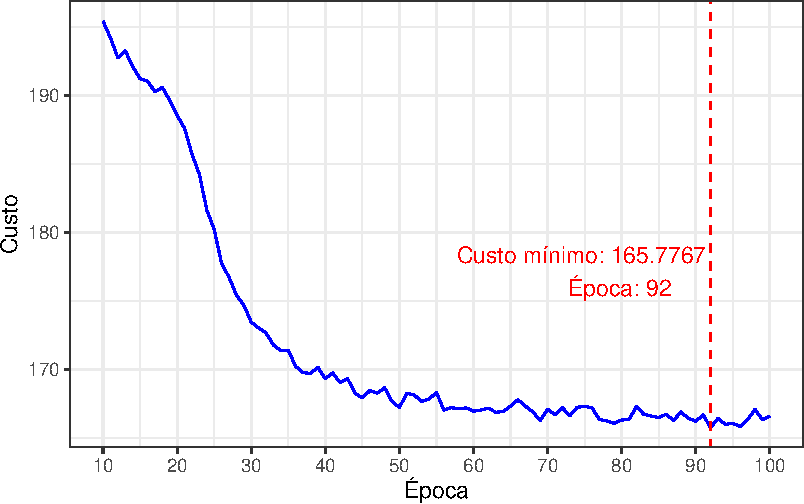
\includegraphics{lista2-resolucao_files/figure-pdf/fig-resultadosq1-1.pdf}

}

\caption{\label{fig-resultadosq1}Custo no conjunto de treinamento}

\end{figure}%

~

O vetor gradiente obtido na melhor época é

\begin{Shaded}
\begin{Highlighting}[]
\NormalTok{best\_grad}
\end{Highlighting}
\end{Shaded}

\begin{verbatim}
       w1        w2        w3        w4        w5        w6        b1        b2 
 1.313836  1.316983 -5.631248 -5.639386  8.835846  8.874542 -2.348411 -2.356765 
       b3 
18.454321 
\end{verbatim}



\end{document}
